
\chapter{Phase Diversity Experiment} 
\label{ch:PDExp}

Here, we will describe the experiment put in place in the optical laboratory at the HEIG-VD to reconstruct wavefronts with unknown static aberrations introduced using phase screens. At first, we study the  behaviour of the phase diversity algorithm put in place by \citet{mugnier_2006} at ONERA with respect to number of averaging images, in other words noise level, and number of Zernike coefficients retrieved. Then we test the algorithm using a known aberration introduced by a parallel plane plate in the beam comparing the result to Zemax simulation. And finally, we introduce the phase screen to have random aberrations in the pupil and try to compare the phase diversity results with the Shack Hartman wavefront sensor results.

\section[ONERA algorithm]{ONERA algorithm, \citet{mugnier_2006}}
\label{sec:ONERAalgo}

In this section, we will briefly present the phase diversity algorithm developed at ONERA since we test and use it to retrieve the phase and the aberrations in the experiment conducted in laboratory.

\subsection{Algorithm description}
\label{subsec:OneraAlgoDesc}

As explained in section \ref{sec:principle}, the phase diversity determines the phase of the wavefront, as well as the unknown object when needed, using two images of the same object with a phase diversity between each image. This gives the following equation system \citep[p.11]{mugnier_2006},

\begin{align}
\mathbf{i}_f &= \mathbf{h}_f \ast \mathbf{o} + \mathbf{n}_f \\
\mathbf{i}_d &= \mathbf{h}_d \ast \mathbf{o} + \mathbf{n}_d,
\label{eqt:systemEQT}
\end{align}

where the bold letters means that it is the sampled quantities, the indexes f and d means respectively focused and defocused and $\mathbf{n}$ regroups the photon and detector noise present on the image. Using the data available, this algorithm approaches the problem at hand with a statistic point of view. They estimate jointly the aberrations and the object \citep{Paxman1992}, which consist to compute the joint maximum \textit{a posteriori} (JMAP) estimator \citep[p.17]{mugnier_2006},

\begin{align}
(\hat{\mathbf{o}},\hat{\boldsymbol{\phi}})_{MAP} &= \underset{\mathbf{o},\boldsymbol{\phi}}{\mathrm{arg \ max}} \ p(\mathbf{i}_f,\mathbf{i}_d,\mathbf{o},\boldsymbol{\phi};\boldsymbol{\theta})\nonumber \\
&= \underset{\mathbf{o},\boldsymbol{\phi}}{\mathrm{arg \ max}} \ p(\mathbf{i}_f|\mathbf{o},\boldsymbol{\phi};\boldsymbol{\theta_n})p(\mathbf{i}_d|\mathbf{o},\boldsymbol{\phi};\boldsymbol{\theta_n})p(\mathbf{o};\boldsymbol{\theta_o})p(\boldsymbol{\phi};\boldsymbol{\theta_{\phi}}), 
\end{align}

where $p(\mathbf{i}_f,\mathbf{i}_d,\mathbf{o},\boldsymbol{\phi};\boldsymbol{\theta})$ is the joint probability density function of the two images $(\mathbf{i}_f,\mathbf{i}_d)$, the object $\mathbf{o}$ and the phase $\boldsymbol{\phi}$. It can also depend on a set of hyperparameters $\boldsymbol{\theta} = (\boldsymbol{\theta}_n,\boldsymbol{\theta}_o,\boldsymbol{\theta}_{\phi})$. $p(\mathbf{i}_k|\mathbf{o},\boldsymbol{\phi};\boldsymbol{\theta_n})$ is the likelihood of the image $\mathbf{i}_k$. $p(\mathbf{o};\boldsymbol{\theta_o})$ and $p(\boldsymbol{\phi};\boldsymbol{\theta_{\phi}})$ are the \textit{a priori} probability density functions of $\mathbf{o}$ and $\boldsymbol{\phi}$.

They assume that the noise is white and stationary with a variance $\sigma^2$ on each image. They take Gaussian prior probability distributions for the object and for the phase which they decompose on the Zernike polynomial basis, $\boldsymbol{\phi}(\mathbf{a})$, with $\mathbf{a}$ the vector containing the Zernike coefficients from $a_4$ to $a_{j_{max}}$, see \citet[p.18-19]{mugnier_2006} for the detailed expressions. Finally, the phase and the object are retrieved by maximizing the joint probability density function $p(\mathbf{i}_f,\mathbf{i}_d,\mathbf{o},\mathbf{a};\boldsymbol{\theta})$ or taking the logarithm of the latter they retrieve them by minimizing the following criterion,

\begin{align}
L&_{JMAP}(\mathbf{o},\mathbf{a},\boldsymbol{\theta}) \nonumber\\
&= -\mathrm{ln} \ p(\mathbf{i}_f,\mathbf{i}_d,\mathbf{o},\mathbf{a};\boldsymbol{\theta}) \nonumber \\
&= N^2\ \mathrm{ln}\ \sigma^2 + \frac{1}{2}\mathrm{ln}\ \mathrm{det}(R_0) + \frac{1}{2}\mathrm{ln}\ \mathrm{det}(R_a)\nonumber\\
& \ + \frac{1}{2\sigma^2}(\mathbf{i}_f -H_f\mathbf{o})^t(\mathbf{i}_f -H_f\mathbf{o})+ \frac{1}{2\sigma^2}(\mathbf{i}_d - H_d \mathbf{o})^t(\mathbf{i}_d-H_d\mathbf{o})\nonumber\\
& \ + \frac{1}{2}(\mathbf{o}-\mathbf{o}_m)^t R_o^{-1}(\mathbf{o}-\mathbf{o}_m) + \frac{1}{2}\mathbf{a}^tR_a^{-1}\mathbf{a} + A,
\end{align}

where $N^2$ is the number of pixels in the image, $\mathbf{o}_m$ and $R_o$ are the mean object and its covariance matrix, $R_a$ is the covariance matrix of the aberrations, $H_k$ is the matrix representing the discrete convolution by the sampled $\mathbf{h}$ and A is a constant.

In order to simplify and fasten the computation, they rewrite the criterion replacing $\mathbf{o}$ by its estimator $\hat{\mathbf{o}}(\mathbf{a},\boldsymbol{\theta})$ obtained by cancelling the derivative of $L_{JMAP}$ with respect to $\mathbf{o}$, and they move to the Fourier domain, see eqt. (24) of \citet[p.21]{mugnier_2006}.

\subsection{Implementation}
\label{subsec:OneraAlgoImp}

The implementation of the algorithm was done by \citet{mugnier_2006}, the code is called \verb!Deco_ConjMarg!. Dr. Laurent Jolissaint wrote the IDL code to run the ONERA phase diversity, it is called \verb!Diversity.pro! and visible in Appendix \ref{subapp:diversity}. The code takes as input an array of at least two PSFs, one focused and one defocused, the $\Delta z$ of the PSFs, the wavelength of the incoming light, the focal distance of the system, the pixel size in arc second, the threshold of the minimization and the mode of reconstruction. It takes also the pupil diameter, pupil central obscuration diameter if needed and finally $j_{max}$. The code can run in two different mode, \textit{Modal} and \textit{Zonal}. The modal method reconstruct the phase using the Zernike basis. The zonal mode uses the pixels of the phase as the basis to reconstruct and the projection on the Zernike is done after the reconstruction. Both method uses the JMAP estimator, but for the zonal I did not find the exact criterion. The modal method uses the criterion presented in section \ref{subsec:OneraAlgoDesc}. 

\section{Experimental Setup}
\label{sec:ExpSetup}

\begin{figure}
\begin{center}
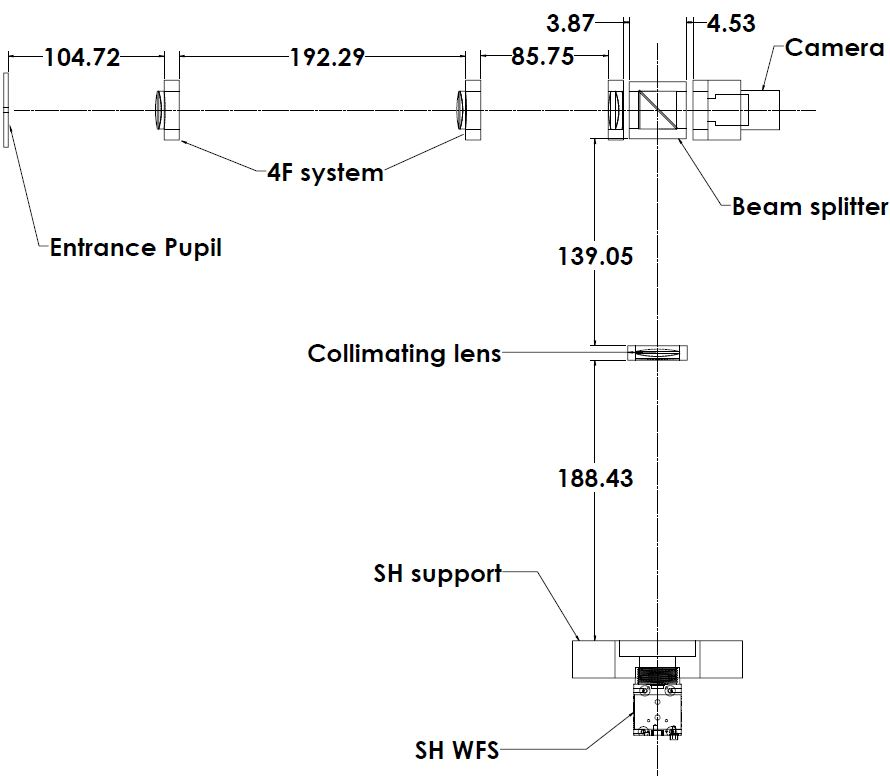
\includegraphics[width=0.8\textwidth,angle=0]{Figures/setupSchema.JPG}
\decoRule
\caption[Experimental Setup Schema]{Experimental setup schema with the relevant distances, \citep{Bouxin_PDM}.}
\label{fig:setupSchema}
\end{center}
\end{figure}

The design of the experiment was already done by \citet{Bouxin_PDM}. The system is built according to her plans and specifications. Figure \ref{fig:setupSchema} shows the schema of the experimental setup.

The experiment is mounted on a pressurized legs optical table. The assembly contains six main components : a light source, an entrance pupil, an imaging system, a converging lens to focus the beam on the camera, a camera and a wavefront sensor.

\subsection{Light source}
\label{subsec:LigthSource}

\begin{minipage}{\linewidth}
\begin{wrapfigure}{r}{0.4\textwidth}
\centering
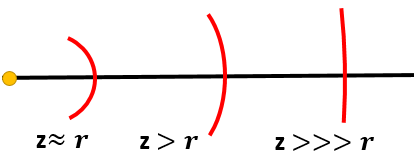
\includegraphics[width=0.4\textwidth]{Figures/WFdistantSource.PNG}
\decoRulewrapFig
\caption[Wavefront curvature]{Wavefront curvature for different point source's distances, \textit{z}. \textit{r} represents the characteristic size of the arc of interest.}
\label{fig:WFdistantSource}
\end{wrapfigure}

The final application of the phase diversity will be to characterize the optical aberrations induced by the imperfect optical path to a scientific detector of a telescope. For this reason, the light source has to simulate a distant star aberration-free wavefront. A distant star wavefront is considered planar since the object distance, z, is far greater than the telescope size, r, see Fig. \ref{fig:WFdistantSource}. The source of our experiment must then be characterized by a planar wavefront.

In order to obtain such a planar wavefront at the entrance pupil, the light source consist of a "pigtailed laser diode", a f=11mm converging lens, a pinhole and a f=200 mm converging lens, see Table \ref{tab:optComp}. The pigtailed laser diode emits a Gaussian beam centred at 637.5 nm slightly diverging. The converging lens concentrates the beam at the center of the 10$\mu$m pinhole to filter the noise. The second converging lens collimates the beam, obtaining a collimated beam with a planar wavefront, see Fig. \ref{fig:sourceRayTracing} and \ref{fig:pinholeEffect}.

\end{minipage}

\begin{figure}
\centering
    \begin{subfigure}{0.5\textwidth}
        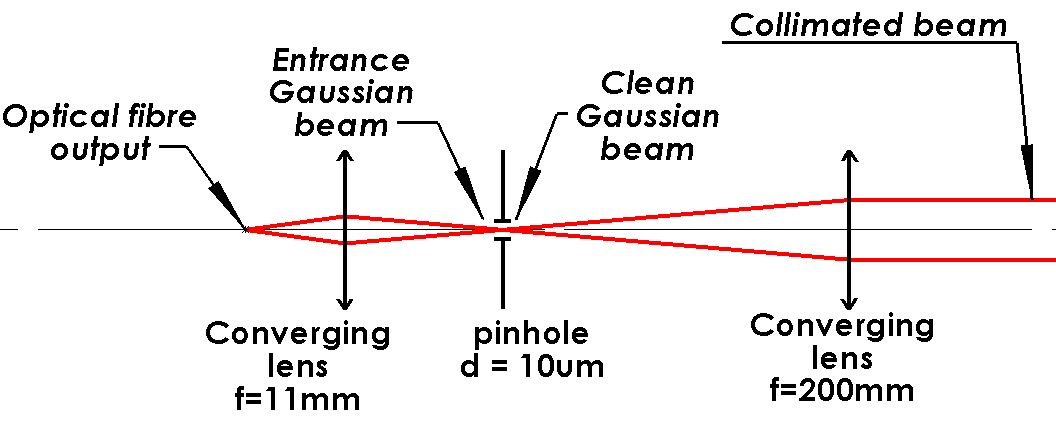
\includegraphics[width=\textwidth]{Figures/source.png}
        \caption{Source ray tracing.}
        \label{fig:sourceRayTracing}
    \end{subfigure}
    \quad
    \begin{subfigure}{0.3\textwidth}
        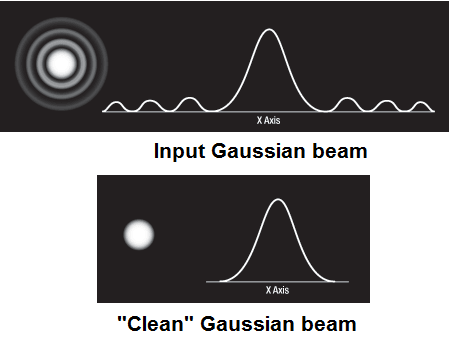
\includegraphics[width=\textwidth]{Figures/pinholeEffect.png}
        \caption{Beam view before and after the pinhole, \citep{SpatialFilters}.}
        \label{fig:pinholeEffect}
    \end{subfigure}
    \decoRule
    \caption{Source schema and pinhole effect on the beam.}
\end{figure}

\subsection{Entrance pupil}
\label{subsec:EntrancePupil}

The entrance pupil of our optical system is a circular aperture of 3.2 mm diameter placed after the collimating lens of the light source. It is milled in a metal plate and centred in his support, to avoid positioning with a XY table. The diameter is chosen in available material to fit in the different detector's surfaces.

\subsection{Pupil imaging system}
\label{subsec:pupilImSystem}

The phase diversity technique requires PSFs images as input, which means that the beam as to be focused onto the detector surface. To analyse the aberration in the pupil plane, one needs to focus an image of the beam passing through the entrance pupil. The simplest assembly to achieve this goal is the 4F system, which consist of two converging lenses of focal 100 mm. The two lenses are separated by 200 mm, see Fig. \ref{fig:setupSchema}. This places the image of the entrance pupil 100 mm after the second converging lens.

\subsection{Detectors}
\label{subsec:Detectors}

The image of the entrance pupil, obtained with the 4F system, is focused onto a CMOS Ximea camera by a f = 80 mm converging lens to acquire the PSFs for the phase diversity wavefront retrieval. The camera has a surface composed by 1280x1024 pixels of 5.3 $\mu$m, see Appendix \ref{app:ximeaCam}. It is mounted on sliding support in order to be able to acquire in/out-of-focus images. A beam splitter is placed in the converging beam to separate it in two. The second beam is collimated and a Shack-Hartman WFS is placed on the entrance pupil image plane, to check the results of the phase diversity wavefront retrieval. The Shack-Hartman WFS has a 39 X 31 lenslets grid and a CCD with a resolution of 1280x1024 pixels of 4.65 $\mu$m, see Appendix \ref{app:SHwfs}. 

\begin{table}
\caption{Optical Components}
\label{tab:optComp}
\centering
\begin{tabular}{|l|l|l|c|}
\hline
\textbf{\#}& \textbf{Components} & \textbf{Model} & \textbf{Reference} \\\hline
1 & Pigtailed laser diode & Thorlabs, LPS-635-FC & \ref{app:pigtailedLaserDiode} \\\hline
2 & Converging lens, f = 11 mm & Thorlabs, A220TM-A & \ref{app:CL11} \\\hline
3 & Pinhole, 10 $\mu$m & Thorlabs, P10S & \ref{app:pinhole10microns} \\\hline
4 & Converging lens, f = 200 mm & Thorlabs, AL100200 & \ref{app:CL200} \\\hline
5 & 3.2 mm Hole milled in metal sheet & ... & ... \\\hline
6 & Converging lens, f = 100 mm & Thorlabs, AC254-100-A & \ref{app:CL100} \\\hline
7 & Converging lens, f = 80 mm & & \\\hline
8 & Camera CMOS & Ximea, MQ013MG-E2 & \ref{app:ximeaCam} \\\hline
9 & Converging lens, f = 100 mm & & \\\hline
10 & Shack-Hartman WFS & Thorlabs, WFS150-5C & \ref{app:SHwfs} \\\hline
\end{tabular}
\end{table}

\section{Data Acquisition}
\label{sec:DataAcquis}

\subsection{Ximea Camera}
\label{subsec:acquisXimCam}

The ONERA algorithm takes at least one focused and one defocused PSFs, as described in section \ref{subsec:OneraAlgoImp}. The PSFs are acquired using a python script which uses an open-source library to control the ximea camera, \verb|pyXimea|\footnote{\url{https://github.com/pupil-labs/pyximea}}, available on GitHub. The acquisition is done following these steps : 

\begin{enumerate}

\item The first step in order to acquire PSFs is to determine the position of the camera's focus point using the python script \verb|AlignementScriptXimeaCamera.py|, see Appendix \ref{subapp:AlignementScriptXimeaCamera}. This script let's you acquire consecutively PSFs at different camera's positions and computes their FWHM. It finally returns the minimum FWHM and the camera's position, see Figure \ref{subfig:28092017AlignementXimeaPSFs} and \ref{subfig:28092017AlignementXimeaPos}.

\begin{figure}
\centering
    \begin{subfigure}{\textwidth}
        \includegraphics[width=\textwidth]{../../../fig/alignement/28092017AlignementXimeaPSFs.png}
        \caption{PSFs taken during the alignment procedure, each image is taken at an other camera position.}
        \label{subfig:28092017AlignementXimeaPSFs}
    \end{subfigure}
    \\
    \begin{subfigure}{0.6\textwidth}
        \includegraphics[width=\textwidth]{../../../fig/alignement/28092017AlignementXimeaPos.png}
        \caption{FWHM of the PSFs as a function of the camera's position. The minimum is at $11.55$ mm}
        \label{subfig:28092017AlignementXimeaPos}
    \end{subfigure}
    \decoRule
    \caption{Example of the results of an alignment procedure}
\end{figure}

\item Once the focus point position of the camera is determined, the acquisition of the data is possible. The acquisition script is called \verb!AcquisAndSaveXimea.py!, see Appendix \ref{subapp:AcquisAndSaveXimea}.

\item The user needs to set the main parameters before acquiring. They are the number of images on which to average, the size of the final PSFs, the position of the focus point on the sliding system and the initial guess to fit the 2D Gaussian on the PSF to find its center. The initial guess can be made using the Ximea camera software, called \verb!xiCamTool!, with which one gets a live feedback of the camera.

\item Then the running program ask the user what he needs to do after having made a sound. The first thing the user needs to do is to place the camera at the focus point and turn on the LED in order to set the optimal exposure time in order to avoid saturation.

\item Finally the acquiring sequence begins, the program ask the user to shut down and turn on the source as the user acquire the different images to get the dark images and the PSF images. The user needs to manually displace the camera to get the defocused PSFs. The program computes the positions to get a $2\pi$ P2V defocus dephasing.

\end{enumerate}

Many functions, used in the two scripts described above, are coded in the script \verb!functionsXimea.py!, see Appendix \ref{subapp:functionsXimea}.

\subsection{Shack-Hartmann WFS}
\label{subsec:acquisSHwfs}

The Shack-Hartmann wavefront sensor is delivered with a software which does the numerical integration to compute
the wavefront. The GUI shows the spot field (focal points), the beam view (irradiance of the
CCD), the wavefront measured or reconstructed (where you can choose the Zernike coefficients
to consider for the integration) and the Zernike coefficients.

\begin{figure}
\begin{center}
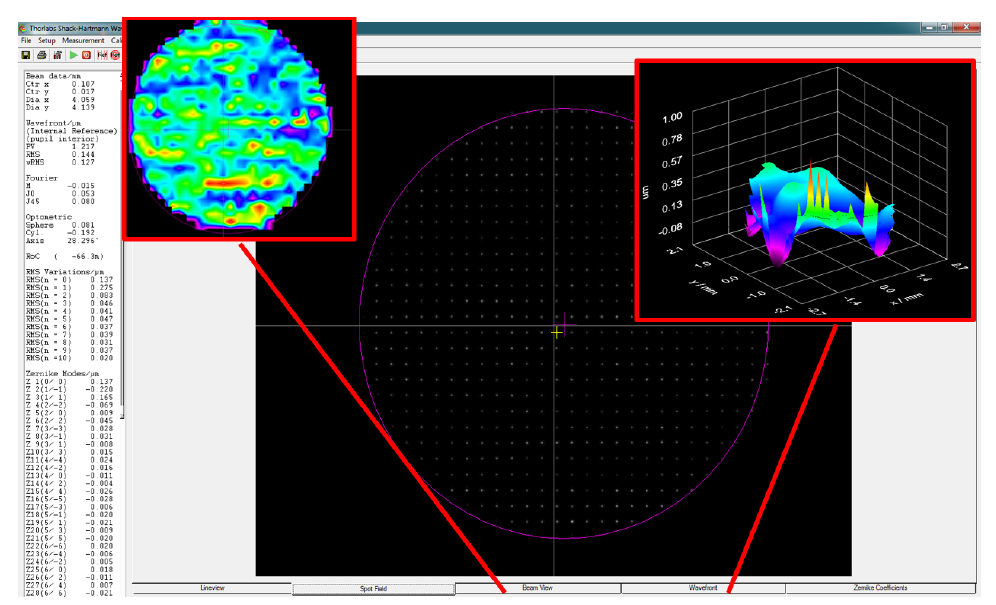
\includegraphics[width=\textwidth,angle=0]{Figures/SHWFS_GUI}
\decoRule
\caption{Shack-Hartmann Software GUI, with the  beam view on the top left, the spot field in the middle and the reconstructed wavefront on the top right.}
\label{fig:}
\end{center}
\end{figure}

The acquisition is done with the company software. The acquired data are the Zernike coefficients and the reconstructed wavefront computed following the principle described in section \ref{subsec:SHprinciple}. Their is a few parameters that the user can set : the exposure time (there is also an auto set), the number of averaging images (1 up to 300) and the focus points reference of the micro-lenses array. 

The data are saved manually in a \textit{.csv} file. I coded an IDL script to read and average the Shack-Hartmann data, in order to be able to analyse them and compare the result with the phase diversity, see Appendix \ref{subapp:readAndAverageSHdata} and \ref{subapp:readSHWFSdata}. 

\section{Results}
\label{sec:Results}

This section presents the results of the phase diversity experiment, with the introduction of different sources of aberration. We will first present the results of the ONERA algorithm test, then we will compare the phase diversity retrieval with a calibrated aberration and finally we will introduce random static aberration with the phase screen and compare the results to the Shack-Hartmann wavefront sensor results.

\subsection{ONERA Phase Diversity test}
\label{subsec:ONERAPDtest}

The motivation of this test is to better understand the behaviour of the ONERA phase diversity algorithm with respect to the different parameters that could influence its results, such as the noise present in the PSFs, the number of Zernike coefficients returned for the modal mode and the error on the position of the Ximea camera.

\begin{figure}
\begin{center}
\includegraphics[width=0.6\textwidth,angle=0]{../../../fig/PD/noise_study/NoiseCurveXimea}
\decoRule
\caption{Noise level as a function of the number of averaging images acquired with $\sim$ 300 $\mu$s exposition time. The noise level is computed as the mean of the standard deviation of every pixel divided by the maximum of the focused PSF.}
\label{fig:NoiseCurve}
\end{center}
\end{figure}

To study the noise, we acquire PSFs with 25 different numbers of averaging images going from 10 to 5000. The noise level is computed as the ratio between the mean pixel standard deviation and the PSF maximum. The Ximea detector has a noise curve visible in Figure \ref{fig:NoiseCurve}. The noise curve is computed with the noise level of the focused PSFs. It follows an exponential law with the number of averaging images. The noise level varies from $\sim 1\mathrm{e}-3$ to $\sim 8\mathrm{e}-5$, for 10 and 5000 images respectively. Having the noise curve of the detector, we can study empirically how it influences the phase diversity results. 

\begin{figure}
\centering
    \begin{subfigure}{\textwidth}
        \includegraphics[width=\textwidth]{../../../fig/PD/noise_study/ZernikeCoef_J_differentNbrAveraging.png}
        \caption{Zernike coefficients $a_j$ as a function of $j$ the Zernike index of the 25 modal and zonal phase retrievals, in blue and red respectively.}
        \label{subfig:ZernikeCoef_J_differentNbrAveragingjmax30}
    \end{subfigure}
    \\
    \begin{subfigure}{0.75\textwidth}
        \includegraphics[width=\textwidth]{../../../fig/PD/noise_study/Boxplot_Aj_j_jmax30.png}
        \caption{Boxplot of the 25 Zernike coefficients $a_j$ of the different phase retrievals computed with the different averaging numbers of images as a function of the Zernike index $j$.}
        \label{subfig:Boxplot_Aj_j_jmax30}
    \end{subfigure}
    \decoRule
    \caption{Results of the phase retrievals computed with the 25 different noise levels. The phase retrievals are done with a $j_{max} = 30$}
\end{figure}

Figures \ref{subfig:ZernikeCoef_J_differentNbrAveragingjmax30} and \ref{subfig:Boxplot_Aj_j_jmax30} presents the results of the 25 different retrievals. As one can see there is some spread due to the different noise levels present in the PSFs given to the algorithm. The biggest standard deviation on a Zernike coefficient is smaller than 6 nm. And there can be up to 20 nm of maximal difference between the $a_j$'s as one can see on Figure \ref{subfig:Boxplot_Aj_j_jmax30}. The spherical aberration, $a_{11}$, has the biggest standard deviation and range of values. This shows that the PSFs noise levels have an impact on the retrieval and that not all Zernike coefficient are affected in the same way. One reassuring point is the good correspondence between the modal and zonal retrievals.

\begin{figure}
\begin{center}
\includegraphics[width=\textwidth,angle=0]{../../../fig/PD/noise_study/WavefrontsNoiseStudy}
\decoRule
\caption{Reconstructed wavefronts for two different numbers of averaging images, 10 and 3500, and their difference are on the first, second and third column respectively. The two first line are modal retrieval with $j_{max}=30$ and $j_{max}=200$ and the last line is the zonal retrieval.}
\label{fig:WavefrontsNoiseStudy}
\end{center}
\end{figure}

Furthermore, looking at the reconstructed wavefronts in Figure \ref{fig:WavefrontsNoiseStudy}, one can see the effect of noise in the PSFs and how important is the choice of $j_{max}$ for the modal reconstruction. Indeed, for the wavefronts reconstructed using $j_{max}=30$, the retrieved structures are similar, however for $j_{max}=200$ there are more structures in the retrieval done on the PSFs with 10 averaging images than with 3500 images. This shows that the noise has a signal at high spatial frequencies. The zonal retrieval shows it clearly, the reconstruction is significantly different between 10 and 3500 averaging images. The averaging over a large number of acquisition smooth out the noise structures that perturbs the reconstruction. Looking at the 25 reconstructed wavefront with the zonal method, the noise threshold is at 3500 averaging images to kill the effect of the noise. Also as said above for the Zernike coefficients and still valid for the wavefront, the two retrieval method gives similar results, as one can compare the three retrievals with 3500 images on the left column of Figure \ref{fig:WavefrontsNoiseStudy}. There is structures present on the wavefront reconstructed on 200 Zernike coefficients, but the footprint of the beam is similar to the two other reconstructions.


\begin{figure}
\begin{center}
\includegraphics[width=\textwidth,angle=0]{../../../fig/PD/noise_study/ZernikeCoef_J_differentJmax_5000Imgs.png}
\decoRule
\caption{Zernike coefficients $a_j$ as a function of $j$ for the 227 retrievals done for 231 different $j_{max}$ from 4 to 231.}
\label{fig:ZernikeCoef_J_differentJmax_5000Imgs}
\end{center}
\end{figure}

In order to be sure that the number of Zernike coefficient retrieved only influenced the wavefront reconstruction and not the $a_j$'s values, we computed them varying $j_{max}$ from 4 to 231 and found that the spread is negligible, see Figure \ref{fig:ZernikeCoef_J_differentJmax_5000Imgs}. This confirmation is expected since the Zernike polynomials are orthonormal, thus not correlated.

\begin{figure}
\centering
    \begin{subfigure}{0.45\textwidth}
        \includegraphics[width=\textwidth]{../../../fig/PD/errorDeltaZStudy/Boxplot_Aj_j.png}
        \caption{Boxplots of the 125 $a_j$'s retrieved with the modal method (blue) and zonal method (red). The PSFs are acquired with 5000 averaging images.}
        \label{subfig:Boxplot_Aj_j}
    \end{subfigure}
    \quad
    \begin{subfigure}{0.45\textwidth}
        \includegraphics[width=\textwidth]{../../../fig/PD/errorDeltaZStudy/Boxplot_stdAj.png}
        \caption{Boxplots of the 125 standard deviations on the Zernike coefficient for the modal and zonal method.}
        \label{subfig:Boxplot_stdAj}
    \end{subfigure}
    \decoRule
    \caption{Results of the $\Delta z$ measurement error test. The plots represent the results of the 125 phase retrievals run with all the permutations of errors, $[-2\sigma,-1\sigma,0,1\sigma,2\sigma]$ with $\sigma = 5\mathrm{e}-3$ mm, on the three PSFs position $\Delta z$}.
\end{figure}

Finally, the last test is to control the impact of a measurement error $\sigma_{\Delta z}$, the error position of the Ximea camera, on the phase retrieval. To do so the latter is run with 125 different permutations of the errors $[-2\sigma,-1\sigma,0,1\sigma,2\sigma]$ on the 3 PSFs position. $\sigma$ is set to represent the best precision we have on the position of the camera. As explained in section \ref{subsec:Detectors}, the camera is mounted on a sliding element moved by a micro metric screw, so $\sigma = 5\mathrm{e}-3$ mm. Figures \ref{subfig:Boxplot_Aj_j} and \ref{subfig:Boxplot_stdAj} present the results. The position error has nearly no effect on the phase retrieval, the median standard deviations are $\sim0.05$ nm and $\sim0.07$ nm for the modal and zonal method respectively.

In conclusion, the ONERA algorithm tests shows that first the two different methods, to retrieve the phase using the JMAP estimator, modal and zonal give similar results. Then, we have seen that the noise levels present in the PSFs influence the retrieval, see Figures \ref{subfig:ZernikeCoef_J_differentNbrAveragingjmax30}, \ref{subfig:Boxplot_Aj_j_jmax30} and \ref{fig:WavefrontsNoiseStudy}. We can consider the noise as an added aberration that touches all the Zernike coefficients. The spherical aberration is the most sensitive one. Also looking at the wavefronts, we see that there is a number of averaging images threshold at 3500 images for the zonal retrieval. Above this threshold the noise seems to be smooth and the retrieval looses the high spatial frequency components. The same thing is true for the modal retrieval, but the smoothing is not as effective at 3500 images. For the rest of this work each PSFs will be acquired with 5000 averaging images. Also we showed that the number of Zernike coefficient $j_{max}$ does not alter the modal retrieval. And finally, the error on the position of the camera also have a negligible impact.

\newpage
\subsection{Parallel plane plate}
\label{subsec:ParPlanePlate}

\begin{figure}
\begin{center}
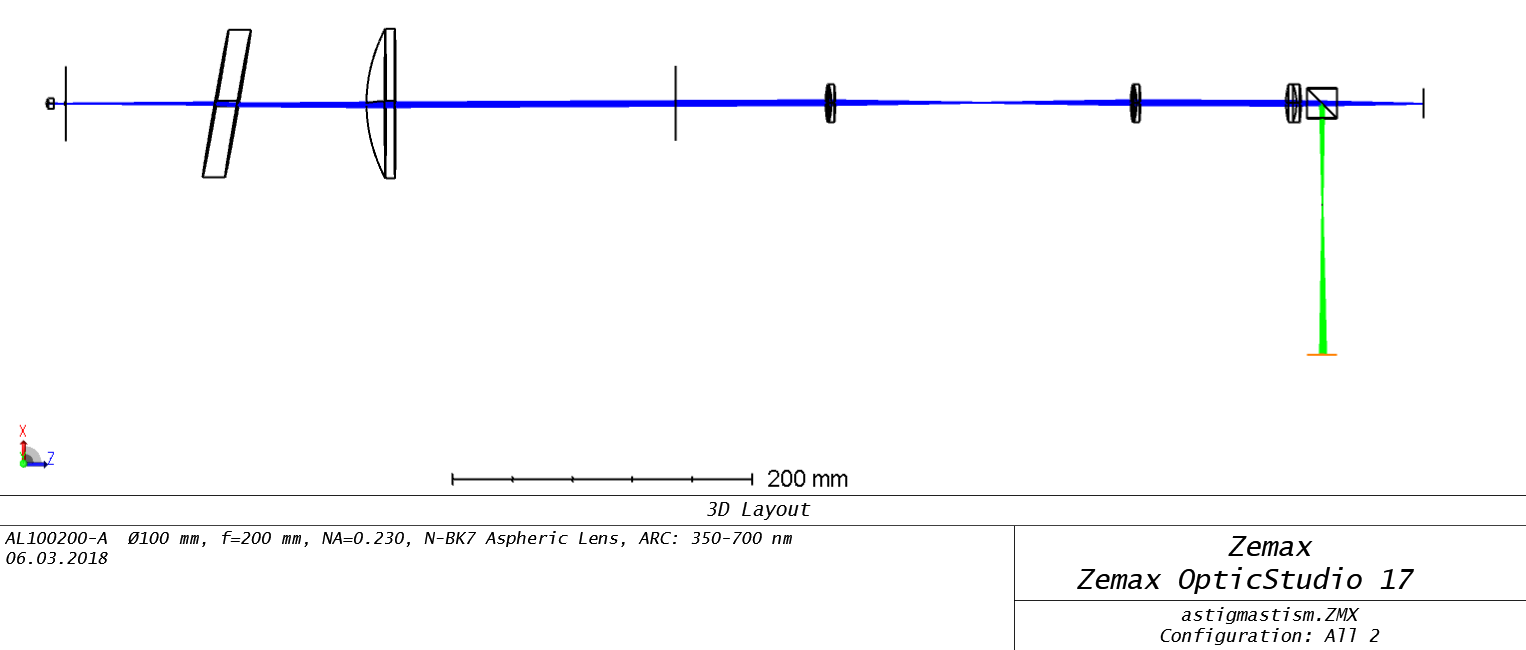
\includegraphics[width=\textwidth,angle=0]{Figures/parallelPlanePlateWithBS.png}
\decoRule
\caption{Zemax simulation of our optical system with the parallel plane plate introducing astigmatism.}
\label{fig:parallelPlanePlate}
\end{center}
\end{figure}

%\begin{minipage}{\linewidth}
%\begin{wrapfigure}{r}{0.5\textwidth}
%\centering
%\includegraphics[width=\textwidth]{}
%\decoRulewrapFig
%\caption{Plexiglas parallel plane plate used to introduce calibrated aberrations.}
%\label{fig:}
%\end{wrapfigure}

Knowing how the algorithm behaves with respect to noise, $j_{max}$, etc... We compare its results to a calibrated aberration. The calibration is computed by simulating the optical system using Zemax\footnote{\url{https://www.zemax.com/opticstudio}}. We introduce astigmatism using a plexiglas parallel plane plate with an angle with respect to the optical axis. The astigmatism comes from the fact that the incident angle is not the same on the left side of the optical axis than on the right side of the optical axis with respect to $x$. This induces a difference in optical path between the symmetrical rays on the left and right side of the optical axis and thus induces an aberration, called the astigmatism.

In order to have the best correspondence between the simulation and the experiment, the results are the difference between the Zernike coefficient of the parallel plane plate and the Zernike coefficient without the plate. Indeed the Zemax simulation do not have alignment issues and other man introduced imperfections. So by subtracting the aberrations present in the system without the parallel plane plate, in theory we should remove any component that do not come from the plate itself in order to only retrieve the plate effect.

\begin{figure}
\begin{center}
\includegraphics[width=0.65\textwidth,angle=0]{../../../fig/PD/astigmatism/angle_study_2/astigmatism_angle.png}
\decoRule
\caption{Zernike coefficient of the vertical astigmatism $a_6$ as a function of the angle of the plexiglas parallel plane plate. The dashed line correspond to the Zemax simulation result, the blue line to the modal retrieval method, the red line to the zonal retrieval and the green line to the Shack-Hartmann reconstruction}
\label{fig:astigmatism_angle_Diversity}
\end{center}
\end{figure}

Figure \ref{fig:astigmatism_angle_Diversity} shows the vertical astigmatism Zernike coefficient $a_6$ as a function of the parallel plane plate angle from $10^{\circ}$ to $50^{\circ}$. The two coloured lines correspond to the two phase retrieval methods and the dashed line is the Zemax simulation of the parallel plane plate. As one can see, there is an offset of $\sim 10-15$ nm between the simulation and the experiment, which correspond to an error of $\sim\frac{\lambda}{64}$. The behaviours of the simulation and the experiment are the same which is reassuring, despite the overestimation of the astigmatism by the phase diversity retrievals. The system without an aberration introduction has a $ a_6 = 2.1$ nm. This might show that our system is not perfectly aligned, but it does explain the $\sim 10-15$ nm offset.

The offset is unexpected, because subtracting the results of the phase retrieval on the PSFs acquired without introducing aberrations to the results with the parallel plane plate should have eliminate the aberration present in the optical system, since the aberration introduction is a linear phenomenon. This might be due to an significant alignment error that could introduce non-linear effect. For instance the alignment of the f=200mm lens that collimates the beam is difficult due to its size and mounting system. One could change it to a f=200mm lens compatible with the 4-rods mounting on which the 4F system is to guaranty the correct alignment. Or that the simulation is not representing exactly the optical system. To go further and try to understand the difference between simulation and experiment, we compare also the coma introduced by the parallel plane plate which should be negligible in the system as shown by the dashed line in Figure \ref{fig:a8astigmatism_angle_Diversity}. The coma is interesting because it is typical in system with alignment problem. In amateur telescopes with two mirrors, it arises when the M2 is not correctly aligned on the M1.

\begin{figure}
\begin{center}
\includegraphics[width=0.65\textwidth,angle=0]{../../../fig/PD/astigmatism/angle_study_2/coma_angle.png}
\decoRule
\caption{Zernike coefficient of the horizontal coma $a_8$ as a function of the angle of the plexiglas parallel plane plate. The dashed line correspond to the Zemax simulation result, the blue line to the modal retrieval method , the red line to the zonal retrieval and the green line to the Shack-Hartmann reconstruction.}
\label{fig:a8astigmatism_angle_Diversity}
\end{center}
\end{figure}

The vertical coma, Zernike coefficient $a_8$, as a function of the parallel plane plate angle is shown in Figure \ref{fig:a8astigmatism_angle_Diversity}. The optical system in presence of the parallel plane plate has a significant coma aberration, up to $\sim15$ according to the phase diversity. Without an aberration introduction, the system has a vertical coma coefficient $a_8=6.4$ nm. All this support the fact that our system is suffering from an alignment problem and that the Zemax simulation is too perfect to be used as a comparison. The only thing really complicated to understand is the non-linearity of the system. It might be do to the fact that the retrieval is done on limited number of Zernike polynomials, $j_{max}=66$ here, which could perturb the retrieval of the wavefront since there is a small spread especially at high spatial frequencies as seen in Figure \ref{fig:ZernikeCoef_J_differentJmax_5000Imgs}. 

\subsection{Shack-Hartmann comparison}

\begin{figure}
\centering
    \begin{subfigure}{0.45\textwidth}
        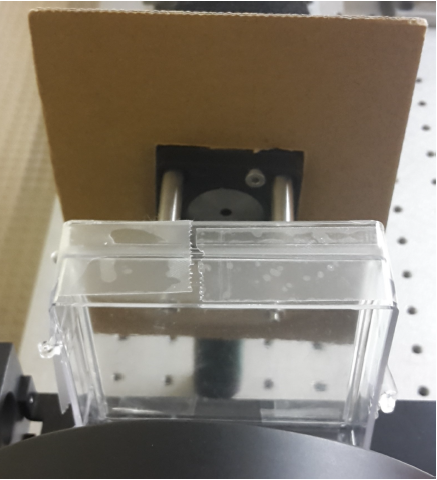
\includegraphics[width=\textwidth]{Figures/phaseScreen}
        \caption{Phase screen used in the experiment.}
        \label{subfig:phaseScreen}
    \end{subfigure}
    \quad
    \begin{subfigure}{0.45\textwidth}
        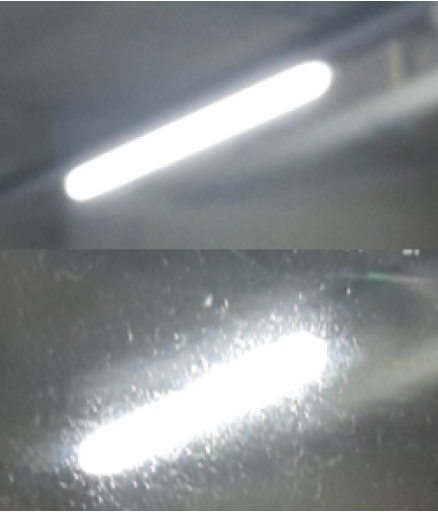
\includegraphics[width=\textwidth]{Figures/StaticTurbulenceEx}
        \caption{Neon light with (up) and without (down) phase screen static turbulence.}
        \label{subfig:StaticTurbulenceEx}
    \end{subfigure}
    \decoRule
    \caption{Phase screen introduction.}
\end{figure}

Even with the problem of calibration, because it is the final aim of the phase diversity experiment, the comparison of the phase diversity and the Shack-Hartmann is done. The phase screen as we call them are transparent plastic boxes, see Figure \ref{subfig:phaseScreen}, whose fabrication process gives them the property of static turbulent aberrations, see Figure \ref{subfig:StaticTurbulenceEx}. Indeed, the plastic injection follows the typical flux that we can find in the atmosphere and the solidification fix the distribution.

\begin{figure}
\begin{center}
\includegraphics[width=0.5\textwidth,angle=0]{../../../fig/PD/phaseScreen/PS2/ZernikeCoef.png}
\decoRule
\caption{Zernike coefficients retrieved as a function of $j$. The red and blue line correspond to the zonal and modal retrieval method respectively. The black line represent the Shack-Hartmann results. $j_{min}=4$ and $j_{max}=66$. }
\label{fig:ZernikeCoef}
\end{center}
\end{figure}

\begin{figure}
\begin{center}
\includegraphics[width=0.5\textwidth,angle=0]{../../../fig/PD/phaseScreen/PS2/Wavefront.png}
\decoRule
\caption{Reconstructed wavefront by the Modal and Zonal method of the phase diversity on 66 Zernike mode on the first line and reconstructed wavefront by the Shack-Hartmann on 66 mode as well, on the second line.}
\label{fig:Wavefront}
\end{center}
\end{figure}

The results of the comparison are presented in Figures \ref{fig:ZernikeCoef} and \ref{fig:Wavefront}. According to both instrument, the phase screen introduces significant aberrations, but the comparison between the two is not satisfying, there is more than 25 nm difference in average between the phase diversity and the Shack-Hartmann. Also the comparison of the wavefronts is not good. The problem is that we do not know which is more cloth to the truth. Indeed, comparing the parallel plane plate results of the Shack-Hartmann and the Zemax model does not help since there is also significant differences between the two, see Figures \ref{fig:astigmatism_angle_Diversity} and \ref{fig:a8astigmatism_angle_Diversity}. However, the vertical coma comparison between the phase diversity and the Shack-Hartmann is better. But we can not really say anything as the astigmatism is completely different. So, it is a shame, but we can not deduct anything with this comparison, at the moment. 

\subsection{Discussion}
\label{subsec:DiscussionOnera}

The results we have gathered in this experiment are mixed. The algorithm test, section \ref{subsec:ONERAPDtest}, is interesting. We learned a lot of things about the properties and behaviour of the ONERA phase diversity algorithm. The noise present in the PSFs has its importance especially when trying to reconstruct the wavefronts. There seems to be a threshold above which the high spatial frequency component of the noise are neutralized. This threshold is at 3500 images corresponding to a noise level of $\sim0.00009$ as observed in the Zonal reconstruction. Also the number of Zernike over which the retrieval is done, $j_{max}$, does not really matters to recover the Zernike coefficient, but as seen in Figure \ref{fig:WavefrontsNoiseStudy} it has a significant influence on the reconstruction of the wavefronts due to the high spatial frequency component of the noise. And also it confirms that a small error of position of the camera would not perturbed the phase retrieval. 

The parallel plane plate experiment used to compare the phase diversity with a calibrated aberration does not work as expected. The astigmatism introduced by the Plexiglas plate follows the right behaviour, but there is an offset that is not expected of $\sim 10-15$ nm. Comparing the vertical coma from the model with the retrieved one, we see that that a significant amount of coma aberration is present even though it is negligible in the Zemax model. Thus we think that there is an alignment problem, moreover the theoretical linearity of the aberration phenomenon in the paraxial approximation is not respected. This non-linearity shows either that the system imperfections and man-introduced aberrations are really high, but it is unlikely as the system seemed fine looking at the collimation, the spot size of the focused beam, etc... or it could show a problem in the use of the ONERA algorithm. It is complicated to conclude with the information at our disposal at the moment.

Finally, in order to improve our results and be able to conclude anything on the ONERA phase diversity algorithm, we would need to be more prudent at the beginning. We should first have a way to describe the system independently, without the phase diversity. It was the idea behind the use of the Shack-Hartmann. But we went to quickly into trying the phase diversity algorithm and testing it. We need to first be sure of the data collected by the Shack-Hartmann, be able to recover the Zemax prediction with the Shack-Hartmann. And once we know how our system behaves and we have a clear way to characterize it, we can try to compare the phase diversity and the Shack-Hartmann.

